\section{Solution}
In this section we will describe some of the technical aspects of creating \name, and discuss the solutions we created to solve the problems we encountered.
\subsection{Modeling}
All objects in our application are simple geometries, such as boxes and spheres, or a collection of multiple geometries. Our train for example consist of multiple boxes and cylinders. To make the game more visually appealing, we used simple texture mapping to apply some fitting textures over the objects. The landscapes we use for the levels in the game are generated using a height map. This is a two dimensional matrix of numbers, in which the row and column map to a coordinate on the flat plan of our world, and the value indicates the height of the terrain on its respective coordinates. The 3D landscape is then rendered by drawing triangles between the height points at each coordinate.
\subsection{Object picking}
In an interactive 3d application, the user will usually need to click on objects to interact with them. The problem of detecting on which object was clicked is called picking, this is a transformation of 2d screen coordinates, to 3d world coordinates. We have solved this problem in the following way.\\
When the user clicks, a ray is cast from the camera position, in the direction in which the camera is pointed. For all objects in our world, we calculate whether this ray collides with the object. This requires of course all objects to have an \emph{intersect} function to determine this. We now have a set of objects the intersect with the ray. For these object, we calculate the distance measured from the camera world coordinates to the first point of intersection. The closest object is then the one that was clicked on.
\subsection{Physics}
Our application requires some sort of physics simulation to determine whether the bridge collide, how the pieces of it interact towards each other and with the environment, etc. Coding a solution ourselves would be very difficult, require a lot of work, and would probably have disappointing results. Therefore we decided to use the JBullet physics library, which can do all physics calculations for us by providing a simple interface. \\
JBullet is used in the following way. Our world consist of objects, simple geometries such as boxes, spheres and cylinders. With JBullet we can create a Rigid Body Control for each geomtetry. We give the RBC the same shape as the geometry, the same position, and we give it a weight. The weight is a float value, which we have to experiment with to get the right feeling for each object, such as the train. When the weight is 0 an object can not move, we used this for the terrain of our world. What JBullet now basically does is calculate the new positions and rotations of each object after a time step. So draw our world with all objects in it, then let JBullet do a step do get the new positions, and draw the world again with the new positions and rotations. To get objects to actually fall, we need to set a gravity value. To get good results for more complex objects, such as the train which consist of multiple cylinders and boxes, we can use a Compound Collision Shape. This way we can construct a Rigid Body from multiple geometries that are connected together. 
\subsection{Collapsing of the Bridge}
JBullet handles collisions between building blocks by looking at the weight and gravity on each building block and this will result in a realistic collapsing bridge. However our bridge is not a solid piece of some material, neither is it a collection of loose blocks. We need some kind of connection, that will break when a certain limit of force on it is exceeded. Luckily this can be done in JBullet using a Joint. A Joint can connect two objects to each other, and the force on a Joint can be calculated by JBullet. So in each time step, we determine the force on each Joint, and if this exceeds some limit, we remove the Joint from the object space, effectively separating the two objects it was connecting. The actual limit at which the joint breaks required some experimenting, but in the end we got a value that had the right results for us; a poor constructed bridge collapsed, and a decent bridge could safely let the train pass.
\subsection{Interface}
We decided to keep the interface very simple. The current interface is shown in \ref{fig:gui}. In this interface only 2 building blocks are available, but we hope to get some more. There are some simple buttons. The two building blocks, the undo button and the play button for letting the train ride over the bridge. By pressing the letter matched to the button, will result in that action too.
\begin{figure}[H]
    \centering
    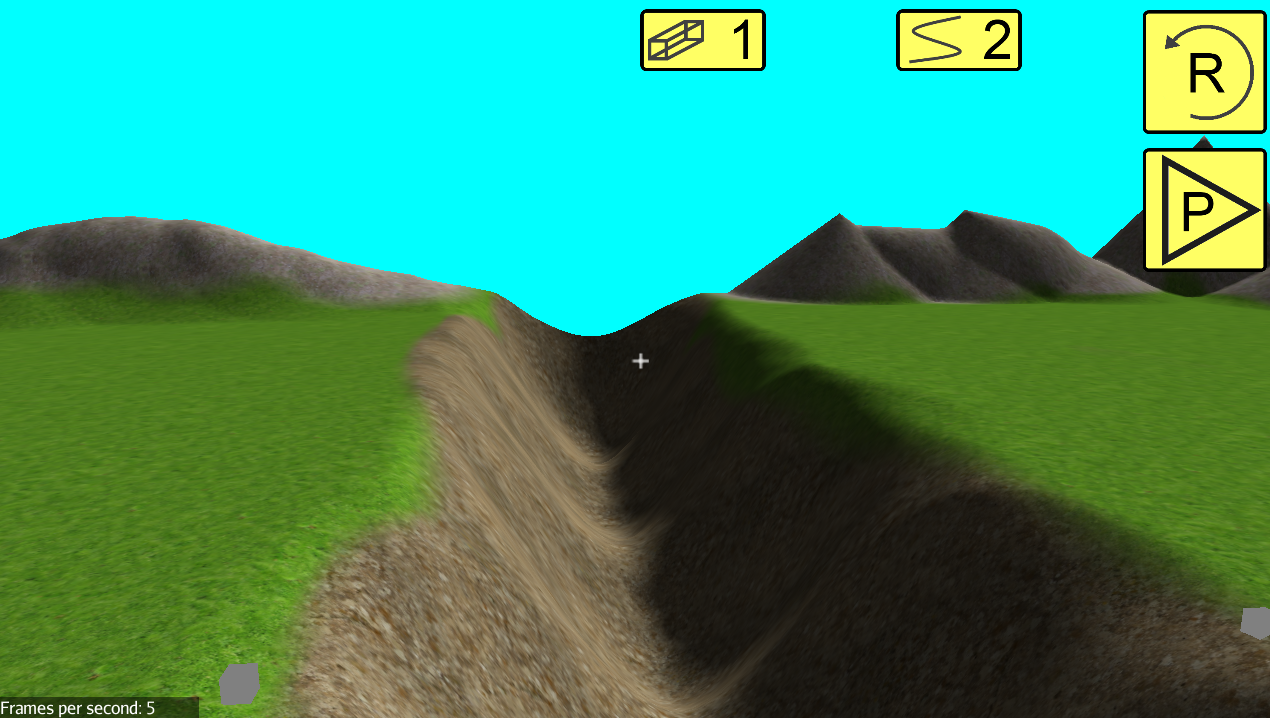
\includegraphics[width=0.8\textwidth]{screenshots/GUI.png}
    \caption{Current interface}
    \label{fig:gui}
\end{figure}
The user can select a point where he wants to connect a building block. This is shown in figure \ref{fig:scp}. When there is a connection point selected, the user can select in which way the building block should be build. This is shown in figure \ref{fig:builded}.
\begin{figure}[H]
    \centering
    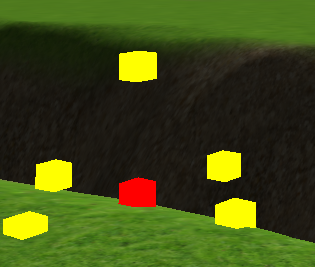
\includegraphics[width=0.4\textwidth]{screenshots/select.png}
    \caption{Selected connection point}
    \label{fig:scp}
\end{figure}
\begin{figure}[H]
    \centering
    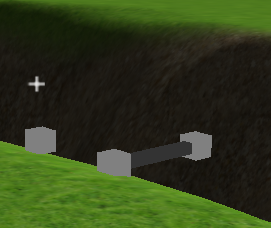
\includegraphics[width=0.4\textwidth]{screenshots/Builded.png}
    \caption{Building block is build}
    \label{fig:builded}
\end{figure}